\section{Method}
\label{sec:method}

\subsection{Diffusion Bridge Implicit Models (DBIM)}
\label{sec:dbim}

\paragraph{Stochastic Bridges.}
Given a base diffusion process $dx_t = f(x_t,t)dt + g(t)dw_t$, the bridge conditioned to reach target $x_0 = \bm{y}$ starting from source $x_T = \bm{x}$ is:
\begin{align}
    dx_t &= f(x_t,t)dt + g(t)dw_t + g(t)^2 \nabla_{x_t} \log p(x_0{=}\bm{y} \mid x_t)\,dt.
\end{align}
Under a variance-preserving (VP) schedule, intermediate states are:
\begin{equation}
    z_t = a_t \bm{x} + b_t \bm{y} + \sigma_t \epsilon, \quad \epsilon \sim \mathcal{N}(0, I),
\end{equation}
where $\bm{x}$ is the source image, $\bm{y}$ is the target image, and $a_t, b_t, \sigma_t$ are schedule coefficients~\cite{zhouDenoisingDiffusionBridge2024}.

\paragraph{Non-Markovian Generalization and Booting Noise.}
We extend the Markovian bridge to a family of non-Markovian processes parametrized by variance $\rho \in \mathbb{R}^{N-1}$. The reverse update rule is:
\begin{equation}
    z_{t_n} = a_{t_n} \bm{x} + b_{t_n} \hat{z}_0 + \sqrt{c_{t_n}^2 - \rho_n^2}\,\hat{\epsilon} + \rho_n \epsilon,
\end{equation}
where $\hat{z}_0 = D_\theta(z_{t_{n+1}}, t_{n+1}, \bm{x})$ is the UNet denoiser prediction. Setting $\rho_n = 0$ gives the deterministic DBIM~\cite{zhengDiffusionBridgeImplicit2025}, analogous to an Euler discretization of a probability-flow ODE over the bridge. Since $c_{t_N} = 0$ leads to a singularity at initialization, we force the first step to be stochastic by setting $\rho_{N-1} = c_{t_{N-1}}$, injecting Gaussian booting noise that encodes the one-to-many mapping ambiguity.

\paragraph{Training Objective.}
The model is trained with Karras-weighted bridge loss:
\begin{equation}
    \mathcal{L} = \mathbb{E}_{(\bm{x},\bm{y}),\,t,\,\epsilon}\bigl[\,w(t) \cdot \|D_\theta(z_t, t, \bm{x}) - \bm{y}\|_2^2\bigr],
    \label{eq:loss}
\end{equation}
where $w(t)$ follows Karras bridge weighting~\cite{karras2022elucidating} and $t$ is sampled from a Karras inverse-$\rho$ distribution.

\paragraph{Architecture.}
Our denoiser $D_\theta$ is a UNet~\cite{ronnebergerUNetConvolutionalNetworks2015} that receives the channel-wise concatenation $[\bm{z}_t, \bm{x}]$ as input. Timestep information is injected via sinusoidal embeddings and Adaptive Group Normalization (AdaGN, ADM-style~\cite{dhariwalDiffusionModelsBeat2021}). The architecture overview is shown in \cref{fig:method_overview}.

For tasks where source and target modalities have different channel counts (e.g., RGB$\rightarrow$IR or SAR$\rightarrow$RGB), we operate the bridge in a shared channel space (typically 3 for RGB-related tasks). Single-band modalities are expanded by channel repetition before entering the UNet, ensuring the concatenation $[\bm{z}_t, \bm{x}]$ remains well-defined across all tasks.

% \vspace{-1em}
\begin{figure}[h]
    \centering
    \includegraphics[page=3,width=\columnwidth]{figures/Figures.pdf}
    \caption{UNet architecture of our DBIM for 1024px tasks (SAR$\rightarrow$RGB, RGB$\rightarrow$IR). We train at 512$\times$512 and infer at full resolution. Source $\bm{x}$ is channel-concatenated with noisy sample $\bm{z}_t$ and processed by this denoiser. Bridge scalings $a_t, b_t, c_t$ construct $\bm{z}_t$ during training; deterministic DBIM sampling generates $\hat{\bm{z}}_0$ during inference.}
    \label{fig:method_overview}
\end{figure}
% \vspace{-1em}

\subsection{Contrastive Unpaired Translation (CUT)}
\label{sec:cut}

For SAR$\rightarrow$IR we use CUT~\cite{parkContrastiveLearningUnpaired2020}: patch-based contrastive learning preserves structure without pixel-aligned pairs. Config: \cref{tab:cut_config}.
